%%%%%%%%%%%%%%%%%%%%%%%%%%%%%%%%%%%%%%%%%
% LaTeX Template
% Version 1.0 
%
% Original authors:
% Hector F. Jimenez S. <hfjimenez@utp.edu.co>
% Brian Ruiz I.		   <brianruiz@utp.edu.co>
% Pereira Security Team 2015.
% License:
% CC BY-NC-SA 3.0 (http://creativecommons.org/licenses/by-nc-sa/3.0/)
%
%----------------------------------------------------------------------------------------
%	PACKAGES AND OTHER DOCUMENT CONFIGURATIONS
%----------------------------------------------------------------------------------------
\documentclass[a4paper]{article}
\usepackage[spanish]{babel}
\usepackage[utf8x]{inputenc}
\usepackage[T1]{fontenc}
\usepackage{amsmath}	
\usepackage{graphicx}
\usepackage{url}
\usepackage{color}
\usepackage{listings}
\usepackage{hyperref}
\hypersetup{
    colorlinks,
    citecolor=black,
    filecolor=black,
    linkcolor=black,
    urlcolor=black
}
\usepackage[export]{adjustbox}
\usepackage{geometry}
 \geometry{
 a4paper,
 total={210mm,297mm},
 	left=30mm,
 	right=20mm,
 	top=20mm,
 	bottom=20mm,
 	bindingoffset=0mm
 }
 
\title{Titulo del Reto }
\author{Correo El\'ectronico \\Nombre}
\begin{document}
\begin{titlepage} 				
\begin{center}	  				
\vfill
\line(1,0){320}\\ 				%Lineas Horizontales.Nombre de Desafio y Reto
\huge\textbf{Space Invaders en DrRacket v0.7}\\	
\large{Héctor F. Jiménez S. - Brian Ruiz I.}\\
\large\texttt{hfjimenez@utp.edu.co - brianruiz@utp.edu.co}\\
\line(1,0){320}\\
\large{Pereira Security Team \\Ingeniería de Sistemas y Computación}
\end{center}
\vspace{4em}
\centerline{
\includegraphics[width=\textwidth]{images/logo}} 			
\begin{center}
\large{Universidad Tecnológica de Pereira \\ 2015 }\\
\end{center}
\vspace{7em}																			%Espacio entre imagen e imagen
\centerline{
\includegraphics[width=\textwidth]{images/slice}} 									%Logo del Reto


\vspace*{\stretch{2.0}}
\end{titlepage}
																			%Pagina En blanco
\clearpage
    \thispagestyle{empty}
    \phantom{a}
    \vfill
    \begin{center}Pagina Dejada Intencionalmente en Blanco\end{center}
    \vfill
\newpage
\tableofcontents
\newpage
\clearpage
%\maketitle
\begin{abstract}
Unidos. Fue lanzado en las máquinas recreativas que funcionan con monedas, el Atari 2600, y la Nintendo Entertainment System. En su vida útil genero más de 500 millones de dólares en ingresos.\\
Es un juego de acción en 2D donde un humano debe proteger la tierra de los extraterrestres. Hay 48 aliens en cada etapa que están uniformemente espaciadas en 6 columnas. Los aliens se mueven hacia izquierda y derecha a través de la pantalla en un patrón establecido, avanzando lentamente hacia la tierra. Es el trabajo del jugador humano disparar a todos los aliens antes de\end{abstract}
\section{Introducci\'on}
Unidos. Fue lanzado en las máquinas recreativas que funcionan con monedas, el Atari 2600, y la Nintendo Entertainment System. En su vida útil genero más de 500 millones de dólares en ingresos.\\
Es un juego de acción en 2D donde un humano debe proteger la tierra de los extraterrestres. Hay 48 aliens en cada etapa que están uniformemente espaciadas en 6 columnas. Los aliens se mueven hacia izquierda y derecha a través de la pantalla en un patrón establecido, avanzando lentamente hacia la tierra. Es el trabajo del jugador humano disparar a todos los aliens antes de
\section{Proposito del Juego}
El juego Space Invaders ha sido un éxito desde que fue lanzado por Taito en 1978. En el plan original para el juego, era que los aliens fueran a matar a soldas humanos. Taito pensó que no querían enviar el mensaje de que disparar a los  seres humanos  estaba bien, así que lo cambiaron a disparar a los aliens.\\
\begin{figure}
  \centering
    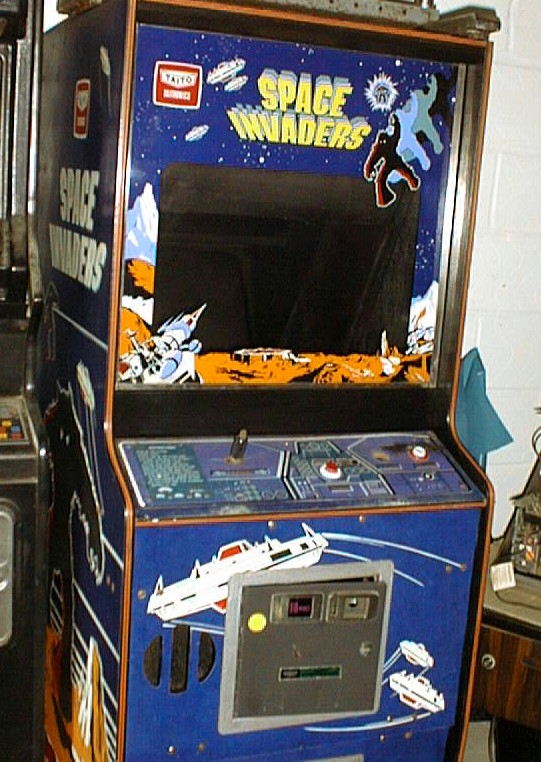
\includegraphics[scale=0.5]{images/machine}
  \caption{Maquina de Space Invaders, Taito 1978.}
  \label{fig:ejemplo}
\end{figure}
Poco después de ser liberado, Space Invaders creció en popularidad. En 1980, se licencia para su uso en los Estados Unidos. Fue lanzado en las máquinas recreativas que funcionan con monedas, el Atari 2600, y la Nintendo Entertainment System. En su vida útil genero más de 500 millones de dólares en ingresos.\\
Es un juego de acción en 2D donde un humano debe proteger la tierra de los extraterrestres. Hay 48 aliens en cada etapa que están uniformemente espaciadas en 6 columnas. Los aliens se mueven hacia izquierda y derecha a través de la pantalla en un patrón establecido, avanzando lentamente hacia la tierra. Es el trabajo del jugador humano disparar a todos los aliens antes de que lleguen a la tierra. Los aliens también disparan al azar, por lo que el jugador humano deben evitar esquivar ser fusilado por los aliens. Si el jugador humano es capaz de destruir los 48 aliens, entonces él o ella avanza a la siguiente etapa en la que tienen un nuevo conjunto de 48 aliens para destruir. Otro aspecto del juego es el conjunto de escudos prestados al jugador. En el juego hay 3 escudos que el jugador humano puede utilizar,  esconderse detrás para evitar recibir un disparo por los extraterrestres. A medida que estos escudos reciben daño, disparos pueden penetrar a través de ellos.\\

Space Invaders se ha actualizado y puesto en libertad en muchas plataformas diferentes, pero todos han sido en forma de dos dimensiones estándar. Hasta el momento Taito nunca ha lanzado una versión en 3D del juego. Sin embargo, en 1999, Space Invaders fue re-lanzado para el Nintendo 64. Aunque los fondos y los personajes fueron diseñados en 3D, el juego sigue siendo un shooter en 2D.

\section{Requisitos para Correr}
Para correr este juego se debe correr con nla opcion Determine Language from Source, para que el archivo del juego 
permita  selesccionar el juego, ademas de ello solo por seguridad puedes incrementar el limite de memoria de 128MB 
a 256MB, es estrictamente necesario que las siguientes lineas se ejecuten:
\begin{lstlisting}[language=python]
(require 2htdp/iamge)  //Importa el paquete de 2htdp image.
(require 2htdp/universe)
(require math)
\end{lstlisting}
El juego se encuentra probado bajo la version 6.2.1 de \textbf{DrRacket} para correr en plataformas Microsoft Windows versiones \textit{ 7,8,8.1,10 Profesional},además  Distribuciones Gnu\/Linux \textbf{\textit{Debian}} y Derivados.
En caso de tener problemas consulte a los desarrolladores.

\section{Detalles Tecnicos de  DrRacket \label{Funciones}}
Para el diseño de este juego y con el fin de poner en practica el concepto de divide and conquer, se crearon las 
siguientes funciones:
\begin{description}
    \item[Comunicador m:] Se encarga de mostrar por pantalla la nave, y enviar los datos a otra funcion denominada \textit{mostrar-balas}
    \item[ver-aliens b:] Se encarga de mostrar los aliens por pantalla, con movimientos.
    \item[monitoreo :]Se encarga de cambiar los valores, también se utiliza para actualizar la posicin de objetos, y crear objetos de manera temporizada. 
    \item[Cambia Posición Aliens:]Actualiza la posición de los aliens dentro de la ventana designada.
    \item[Mouse] Maneja la posicion de la nave utilizando el mouse, las posiciones de esta solo son en 1d 
        en el eje X, descarta las posicion del mouse en Y,Z.
\end{description}
\subsection{Creacion de Ventanas}

\subsection{Funciones de Movimiento}
No olvide Incluir Imagenes.
%http://www.laqee.unal.edu.co/tex-archive/info/epslatex/english/epslatex.pdf
%\begin{figure}
%  \centering
%    \includegraphics{grafico}
%  \caption{Mi Figura}
%  \label{fig:ejemplo}
%\end{figure}

\subsection{Funciones de Disparo}
No olvide Incluir Imagenes.
\subsection{Funciones de Dificulta}
asdasdas
\subsection{Funciones de Sonido}

\clearpage
\newpage
%Toolset.
\section{Links de Paginas de Interés \label{Herramientas}}
\begin{itemize}
\item \href{http://virtualbox.org}{Virtualbox}
\item \href{www.wireshark.org}{Wireshark}
\item \href{www.wireshark.org}{Terminal Based Wireshark}
\item \href{http://www.gnu.org/software/coreutils/}{Coreutils}
\item \href{http://www.secdev.org/projects/scapy/}{Scapy}
\item \href{http://www.chiark.greenend.org.uk/~sgtatham/putty/}{PuTTY}
\clearpage
\newpage
\section{Adjuntos}
Archivos Adjuntos: Scripts, Pruebas\ldots etc 
\clearpage
\newpage
\section{Agradecimientos}
Agradecimientos en esta seccion \href{http://www.ejemplourl.org}{Ejemplo URL} 

\end{itemize}
\end{document}
